% Created 2016-08-17 Wed 14:38
\documentclass[tikz]{standalone}
\usepackage[utf8]{inputenc}
\usepackage[T1]{fontenc}
\usepackage{helvet}
\renewcommand{\familydefault}{\sfdefault}
\usepackage{tikz}
\author{Holger Karl}
\date{\today}
\title{}
\begin{document}
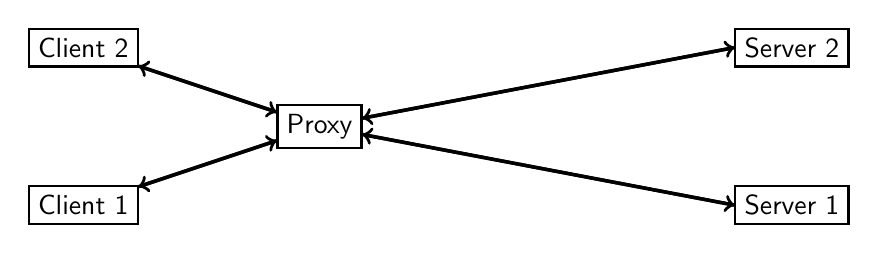
\begin{tikzpicture}[auto, xscale=3,
block/.style = {rectangle, draw=black, thick, align=left}]
\node[block] at (0,0) (c1) {Client 1};
\node[block] at (0,2) (c2) {Client 2}; 
\node[block] at (1,1) (pr) {Proxy}; 
\node[block] at (3,0) (s1) {Server 1}; 
\node[block] at (3,2) (s2) {Server 2}; 
\draw [->] (c1)  [line width=1.25] -- (pr); 
\draw [->] (c2) [bend left=45, line width=1.25] -- (pr); 
\draw [->] (pr)  [line width=1.25] -- (c1); 
\draw [->] (pr) [line width=1.25] -- (c2); 
\draw [->] (pr) [line width=1.25] -- (s1.west); 
\draw [->] (s1.west) [line width=1.25] -- (pr); 
\draw [->] (pr) [line width=1.25] -- (s2.west); 
\draw [->] (s2.west) [line width=1.25] -- (pr); 
  % \node [block]  at (0,1) (sender) {\textbf{Sender:} \\x = native data;\\px = pack(x);
  %   \\send(px);};
  % \node [block] at (2,3) (idl) {Data definition file};
  % \node [block] at (2,2) (idlcomp) {IDL compiler};
  % \node [block] at (1,1) (pack) {pack()}; 
  % \node [block] at (3,1) (unpack) {unpack()}; 
  % \node [block]  at (4,1) (receiver) {\textbf{Receiver:} \\px =  receive();\\x = unpack(px);
  %   \\//use native data in x };
  % %
  % \draw [->] (idl) -- (idlcomp); 
  % \draw [->] (idlcomp) -- (pack); 
  % \draw [->] (idlcomp) -- (unpack); 
  % \draw (-1,-1) -- (5,-1);
  % \draw [->] (sender) -- (0, -1); 
  % \draw [->] (4, -1) -- (receiver); 
  % \draw  [->] (sender.east) -- [bend left=80] (pack.west) ; 
  % \draw  [->] (pack.west) -- [bend left=45] (sender.east) ; 
  % \draw  [->] (receiver.west) -- [bend left=45] (unpack.east) ; 
  % \draw  [->] (unpack.east) -- [bend left=45] (receiver.west) ; 
  % \path (sender) edge [bend north ] node [right] {} (pack);
\end{tikzpicture}
\end{document}